
\chapter{Synchronous context free grammars} \label{sec:scfg}

%\subsubsection*{Synchronous context free grammar} \label{sec:scfg}
\begin{figure}[t]
\begin{center}
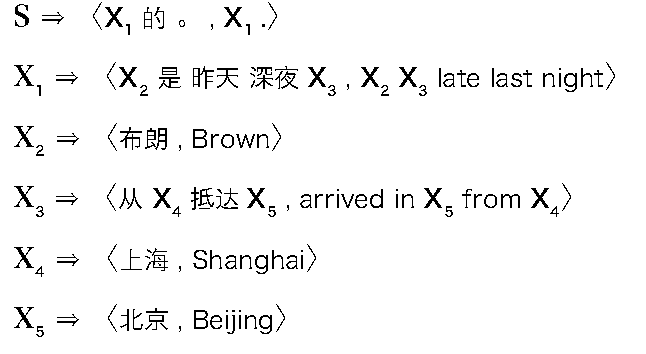
\includegraphics[width=0.6\columnwidth]{example_derivation2.pdf}
\end{center}
\caption[Derivation]{An example SCFG derivation from a Chinese source sentence which yields the English sentence: {\em ``Brown arrived in Shanghai from Beijing late last night.''}. The non-terminal alignment $\mathbf{a}$ is specified by the variable subscripts.}
\label{fig:intro_example_derivation}
\end{figure}

The translation models discussed explored in this workshop are based on synchronous grammars. 
Here we provide a short definition of the formalism we've employed: synchronous context free grammar (SCFG).

A synchronous context free grammar (SCFG, \cite{lewis68scfg}) generalizes context-free grammars to generate strings concurrently in two (or more) languages. A string pair is generated by applying a series of paired rewrite rules of the form, $X \rightarrow \langle \mathbf{e}, \mathbf{f}, \mathbf{a} \rangle$, where $X$ is a non-terminal, $\mathbf{e}$ and $\mathbf{f}$ are strings of terminals and non-terminals and $\mathbf{a}$ specifies a one-to-one alignment between non-terminals in $\mathbf{e}$ and $\mathbf{f}$.
In the context of SMT, by assigning the source and target languages to the respective sides of a probabilistic SCFG it is possible to describe translation as the process of parsing the source sentence, which induces a parallel tree structure and translation in the target language \cite{chiang07hierarchical}.  
Terminal are rewritten as pairs of strings of terminal symbols in the source and target languages.  Additionally, one side of a terminal expansion may be the special symbol $\epsilon$, which indicates a null alignment which permits arbitrary insertions and deletions.
Figure \ref{fig:intro_example_derivation} is an example derivation for Chinese to English translation using an SCFG of the form that I propose to learn using non-parametric Bayesian models.

The generative story is as follows. 
In the beginning was the grammar, in which we allow  two types of rules: {\emph non-terminal} and {\emph terminal} expansions. 
The former rewrites a non-terminal symbol as a string of two or three non-terminals along with an alignment $\mathbf{a}$, specifying the corresponding ordering of the child trees in the source and target language. 
Terminal expansion rewrite a non-terminal as a pair of terminal n-grams, where either but not both may be empty. 
Given a grammar, each sentence is generated as follows, starting with the distinguished root non-terminal, $S$. 
Rewrite each frontier non-terminal, $c$, using a rule chosen from our grammar expanding $c$. 
Repeat until there are no remaining frontier non-terminals. 
The sentences in both languages can then be read off the leaves, using the rules' alignments to find the right ordering. 

\begin{figure}[t]
  \centering
  \subfigure{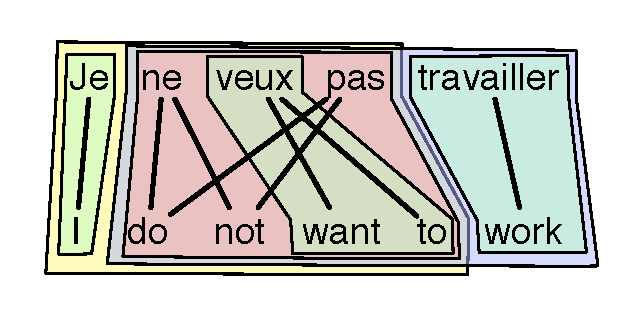
\includegraphics[scale=0.7]{intro_slides/PhraseExtraction1.pdf}}
  \subfigure{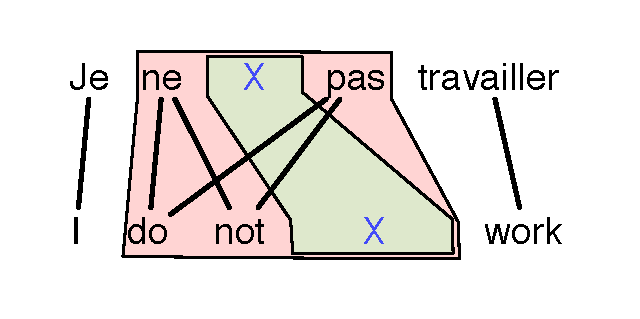
\includegraphics[scale=0.7]{intro_slides/HieroExtraction2.pdf}}
\caption{Extracting translation rules from aligned sentences. All the phrases obtained using the standard phrase extraction heuristics are depicted in the left figure, these are: $\langle$ Je, I $\rangle$, $\langle$ veux, want to $\rangle$, $\langle$ travailler, work $\rangle$, $\langle$ ne veux pas, do not want to $\rangle$, $\langle$ ne veux pas travailler, do not want to work $\rangle$, $\langle$ Je ne veux pas, I do not want to $\rangle$, $\langle$ Je ne veux pas travailler, I do not want to work $\rangle$. On the right is shown how a discontiguous SCFG rule is created by generalising a phrase embedded in another phrase, the extracted rule is: X $\rightarrow$ $\langle$ ne X$_1$ pas, do not X$_1$ $\rangle$.}
\label{fig:intro_rule_extraction}
\end{figure}

The process for extracting SCFG rules is based on that used to extract translation phrases in phrase based translation systems. 
The phrase based approach \cite{koehn03} uses heuristics to extract phrase translation pairs from a word-aligned corpus. 
The phrase extraction heuristic is illustrated in Figure \ref{fig:intro_rule_extraction}. 
This heuristic extracts all phrases whose words are either not aligned, or aligned with only other words in the same phrase. 
The phrase translation probabilities are then calculated using a maximum likelihood estimation. 

The Hiero \cite{chiang07hierarchical} SCFG extraction heuristic starts from a grammar consisting of the set of contiguous phrases, wherever a phrase is wholly embedded within another a new rule is add with the embedded phrase replace by the non-terminal X. 
This process continues until all possible rules have been extracted, subject to the constraints that every rule must contain a terminal on the source side, a rule may only contain two non-terminals on its right side and that those non-terminals may not be adjacent.
The left example in Figure \ref{fig:intro_rule_extraction} depicts this rule generalisation process. 
